\documentclass[a4paper,12pt]{article}
\usepackage{graphicx}
\usepackage{bm,amssymb}
\usepackage{mathrsfs}
\usepackage[unicode,colorlinks=true,filecolor=blue, menucolor=black, linkcolor=black, citecolor=black,pagebackref=white]{hyperref}
\usepackage[utf8]{inputenc}
\usepackage[russian]{babel}
\usepackage{amsmath}
\usepackage{caption}
\usepackage[left=2cm,right=2cm, top=2cm,bottom=2cm,bindingoffset=0cm]{geometry}
\begin{document}
\title{Семинар по теме: <<Преобразование Фурье>>}
\maketitle


\subsection*{Интеграл Фурье}

Если есть функция $f(x)$, $x\in\mathbb{R}$, то для неё можно определить
разложение в интеграл Фурье (так называемое обратное преобразование
Фурье):

\[
f\left(x\right)=\int_{-\infty}^{\infty}\tilde{f}(p)e^{ipx}\frac{dp}{2\pi}
\]


\noindent
При этом функцию $\tilde{f}\left(p\right)$ можно получить, используя
прямое преобразование Фурье:
\[
\tilde{f}(p)=\int_{-\infty}^{\infty}f(x)e^{-ipx}dx
\]


\noindent
Согласованность двух формул обеспечивается следующим выражением для
$\delta$-функции:
\[
\int_{-\infty}^{\infty}e^{ipx}dp=2\pi\delta\left(x\right)
\]


\noindent
Напомним, $\delta$-функция определяется как функция, такая, что для
любой функции $f(x)$ выполнено:

\[
\int_{-\infty}^{\infty}\delta(x)f(x)dx=f(0)
\]



\subsubsection*{Замечание}

В разных источниках преобразование Фурье вводится по-разному. Например,
в прямом преобразовании Фурье вместо $e^{-ipx}$ можно написать $e^{ipx}$;
в таком случае аналогичную замену нужно проделать и в обратном преобразовании
Фурье; соотношения по-прежнему останутся согласованными. Кроме того,
в математике часто рассматривается преобразование Фурье, в котором
в интегралах вместо $dx$ и $\frac{dp}{2\pi}$ стоит $\frac{dx}{\sqrt{2\pi}}$
и $\frac{dp}{\sqrt{2\pi}}$; допустим любой выбор констант, лишь бы
их произведение было $2\pi$.


\subsection*{Ряд Фурье}

Если есть функция $f(x)$, периодичная с периодом $T$ (или просто
определенная на отрезке длиной $T$; в таком случае ее можно просто
периодически продолжить), то для этой функции можно определить разложение
в ряд Фурье:
\[
f(t)=\sum_{n=-\infty}^{\infty}f_{n}e^{i\omega_{n}t}
\]


\noindent
Периодичность функции обеспечивается требованием на частоты $\omega_{n}T=2\pi n$.
Коэффициенты ряда Фурье можно получить из соотношения
\[
f_{n}=\frac{1}{T}\int_{0}^{T}f(t)e^{-i\omega_{n}t}dt
\]


\noindent
Согласованность разложения в ряд Фурье обеспечивается следующим тождеством
(тождество Пуассона):
\[
\sum_{n=-\infty}^{\infty}\delta(t+nT)=\frac{1}{T}\sum_{n=-\infty}^{\infty}e^{i\omega_{n}t}
\]



\subsubsection*{Замечание}

Тут тоже имеется произвол в выборе знаков в экспоненте (лишь бы они
были разные) и в коэффициентах перед интегралом и рядом (лишь бы их
произведение равнялось $T$).


\subsection*{Ряд Фурье для решёточных функций}

Если есть исходная функция, определенная на решётке (то есть, на самом
деле, она представляет собой обычную числовую последовательность)
$f_{n}$, $n\in\mathbb{Z}$. В таком случае, можно рассмотреть преобразование,
аналогичное предыдущему, только в ``обратном'' направлении. А именно,
можно рассмотреть разложение $f_{n}$ по плоским волнам в виде
\[
f_{n}=\int_{-\pi}^{\pi}f(k)e^{ikn}\frac{dk}{2\pi}
\]


\noindent
и выражение для $f(k)$ ($k\in\left[-\pi;\pi\right]$) даётся выражением:
\[
f(k)=\sum_{n=-\infty}^{\infty}f_{n}e^{-ikn}
\]


\noindent
Это преобразование полностью аналогично предыдущему, и его согласованность
тоже обеспечивается тождеством Пуассона.


\subsection*{Дискретное преобразование Фурье}

Если есть исходный набор из $N$ чисел $f_{n}$, $n=1,\dots,N$, то
для него можно определить дискретное преобразование Фурье. Оно представляет
собой разложение по дискретному набору плоских волн:
\[
f_{n}=\sum_{k}\tilde{f}_{k}e^{ikn}
\]


\noindent
при этом волновой вектор $k_{m}=\frac{2\pi}{N}m$ и $m=1,\dots,N$;
под $\sum_{k}f\left(k\right)$ подразумевается $\sum_{m=1}^{N}f\left(k_{m}\right)$.
При этом обратное преобразование Фурье даётся выражением
\[
\tilde{f}_{k}=\frac{1}{N}\sum_{n=1}^{N}f_{n}e^{-ikn}
\]


\noindent
Согласованность дискретного преобразования Фурье обеспечивается следующим
тождеством:
\[
\sum_{k}e^{ikn}=N\delta_{n0}=\begin{cases}
N, & n=0\\
0, & n\neq0
\end{cases}
\]



\subsubsection*{Замечание}

Интересно, что разложение в ряд Фурье можно получить как предел $N\to\infty$
у дискретного преобразования Фурье; а разложение в интеграл Фурье
можно получить как предел $T\to\infty$ разложения в ряд Фурье. Таким
образом, все эти преобразования получаются друг из друга.


\subsection*{Задача 1 (Потенциал Юкавы или потенциал Дебая)}

В рамках Стандартной Модели возникает так называемое взаимодействие
Юкавы. Если имеется точечная частица, несущая ``заряд'' $q$ и расположенная
в начале координат, то оказывается, что потенциал, создаваемый этим
зарядом (аналог электрического потенциала) удовлетворяет уравнению
\[
-\Delta\varphi(\mathbf{r})+\kappa^{2}\varphi(\mathbf{r})=4\pi q\cdot\delta(\mathbf{r})
\]


\noindent
где $\Delta\varphi\equiv\frac{\partial^{2}\varphi}{\partial x^{2}}+\frac{\partial^{2}\varphi}{\partial y^{2}}+\frac{\partial^{2}\varphi}{\partial z^{2}}$
- оператор Лапласа; $\kappa$ - некий параметр задачи. Решим это уравнение,
найдём потенциал.


\subsubsection*{Решение}

Исходное однородное уравнение (без правой части) удовлетворяет требованию
трансляционной инвариантности (то есть - если провести в уравнении
замену $\mathbf{r}\rightarrow\mathbf{r}+\mathbf{a}$, где $\mathbf{a}$
- произвольный вектор, то уравнение не изменится); это значит, что
его можно решать при помощи преобразования Фурье.

\noindent
Подставим в уравнение $\varphi(\mathbf{r})$ в виде (обратное преобразование
Фурье):
\[
\varphi(\mathbf{r})\equiv\varphi(x,y,z)=\iiint\varphi(p_{x},p_{y},p_{z})e{}^{ip_{x}x+ip_{y}y+ip_{z}z}\frac{dp_{x}}{2\pi}\frac{dp_{y}}{2\pi}\frac{dp_{z}}{2\pi}\equiv\int\frac{d^{3}\mathbf{p}}{(2\pi)^{3}}\varphi(\mathbf{p})e^{i\mathbf{p}\mathbf{r}}
\]


\noindent
(тут для удобства функцию $\varphi(\mathbf{r})$ и её фурье-образ
$\varphi(\mathbf{p})$ мы обозначаем одинаково; чтобы их различать,
будем иметь в виду, что когда аргумент функции - $\mathbf{p}$, то
имеется в виду фурье-образ, а когда аргумент - $\mathbf{r}$, то имеется
в виду сама функция). В таком случае, все дифференцирования, содержащиеся
в операторе Лапласа, можно ``пронести'' под знак интеграла, где
они будут действовать только на экспоненту как $\frac{\partial}{\partial x}e^{i\mathbf{p}\mathbf{r}}=ip_{x}e^{i\mathbf{p}\mathbf{r}}$.
Таким образом, можно сразу записать:
\[
\Delta\varphi(\mathbf{r})=\int\frac{d^{3}\mathbf{p}}{\left(2\pi\right)^{3}}\varphi(\mathbf{p})(-\mathbf{p}^{2})e^{i\mathbf{p}\cdot\mathbf{r}}
\]


\noindent
По свойству $\delta$-функции, правую часть можно тоже представить
в виде преобразования Фурье от константы:
\[
4\pi q\delta(\mathbf{r})=4\pi q\int\frac{d^{3}\mathbf{p}}{(2\pi)^{3}}e^{i\mathbf{p}\cdot\mathbf{r}}
\]


\noindent
А значит, уравнение запишется как:
\[
\int\frac{d^{3}\mathbf{p}}{(2\pi)^{3}}(\mathbf{p}^{2}+\kappa^{2})\varphi(\mathbf{p})e^{i\mathbf{p}\cdot\mathbf{r}}=\int\frac{d^{3}\mathbf{p}}{(2\pi)^{3}}4\pi q\cdot e^{i\mathbf{p}\cdot\mathbf{r}}
\]


\noindent
А теперь мы можем провести преобразование Фурье этого выражения. В
данном уравнении это равносильно условному ``сокращению'' операции
$\int\frac{d^{3}\mathbf{p}}{\left(2\pi\right)^{3}}e^{i\mathbf{p}\cdot\mathbf{r}}\dots$
слева и справа. Таким образом, для Фурье-образа $\varphi(\mathbf{p})$
получается тривиальное скалярное уравнение:
\[
\varphi(\mathbf{p})(\mathbf{p}^{2}+\kappa^{2})=4\pi q\Rightarrow\varphi(\mathbf{p})=\frac{4\pi q}{\mathbf{p}^{2}+\kappa^{2}}
\]


\[
\varphi(\mathbf{r})=\int\frac{d^{3}\mathbf{p}}{(2\pi)^{3}}\varphi(\mathbf{p})e^{i\mathbf{p}\mathbf{r}}=\int\frac{d^{3}\mathbf{p}}{(2\pi)^{3}}\frac{4\pi q}{\mathbf{p}^{2}+\kappa^{2}}e^{i\mathbf{p}\mathbf{r}}
\]


\noindent
Этот интеграл можно взять, перейдя к сферическим координатам. Азимутальный
угол $\theta$ мы будем отсчитывать от направления вектора $\mathbf{r}$.
Как мы знаем из предыдущих семинаров, якобиан перехода к сферическим
координатам выглядит как $d^{3}\mathbf{p}=p^{2}dp\sin\theta d\theta d\varphi$.
Таким образом:
\begin{multline*}
\varphi(\mathbf{r})=\frac{1}{(2\pi)^{3}}\int_{0}^{\infty}p^{2}dp\int_{0}^{\pi}\sin\theta d\theta\int_{0}^{2\pi}d\varphi\frac{4\pi q}{p^{2}+\kappa^{2}}e^{ipr\cos\theta}=\\
=\frac{2q}{\pi}\int_{0}^{\infty}p^{2}dp\cdot\frac{\sin(pr)}{pr}\cdot\frac{1}{p^{2}+\kappa^{2}}=\frac{2q}{\pi r}\int_{0}^{\infty}\frac{z\sin z}{z^{2}+\kappa^{2}r^{2}}dz=\frac{q}{r}e^{-\kappa r}
\end{multline*}


\noindent
Тут мы взяли сперва интеграл по $\varphi$ и $\theta$, затем обезразмерили
интеграл по $p$ и воспользовались интегралом Лапласа из 4 семинара.
Полученный ответ совпадает с законом Кулона на малых расстояниях $r\ll\frac{1}{\kappa}$;
на больших расстояниях возникает эффект экранирования. Аналогичное
явление возникает в плазме, при внесении в неё электростатического
заряда $q$. Явление это называется дебаевским экранированием, параметр
$\frac{1}{\kappa}$ в этой модели называется дебаевским радиусом.
Сам же потенциал тоже иногда называется дебаевским.


\subsection*{Задача 2}

Пусть имеется грузик на пружинке (осциллятор), который возмущаяется
периодической внешней силой $F(t)$. Уравнение движения запишется
в таком случае как:
\[
\ddot{x}(t)+\omega^{2}x(t)=f(t)
\]


\noindent
(где $f(t)=\frac{1}{m}F(t)$ и $\omega^{2}=\frac{k}{m}$). Внешняя
сила имеет период $T$ и имеет вид ``прямоугольников'': сперва в
течении первой половины периода, грузик ``тянут'' в одну сторону,
а затем - в другую:
\[
f(t)=\begin{cases}
-f_{0} & -\frac{T}{2}<t<0\\
f_{0} & 0<t<\frac{T}{2}
\end{cases}
\]


\noindent
Исследуем отклик осциллятора на такую периодическую силу. Решим задачу
с начальными условиями $x\left(0\right)=0$, $\dot{x}(0)=0$.


\subsubsection*{Решение}

В силу однородности по времени уравнения без правой части (однородность
и трансляционная инвариантность - это одно и то же), различные гармоники
(колебания с различными частотами) будут жить независимо.

\noindent
Значит, для исследования уравнения нужно представить возмущающую силу
$f\left(t\right)$ в виде разложения в ряд Фурье. Поскольку функция
имеет период $T$, то разложение будет содержать лишь гармоники $\omega_{n}T=2\pi n\Rightarrow\omega_{n}=\frac{2\pi}{T}n$.
Получаем:
\[
f(t)=\sum_{n=-\infty}^{\infty}f_{n}e^{-i\omega_{n}t}
\]


\noindent
в таком случае коэффициенты ряда Фурье будут выражаться как:
\begin{multline*}
f_{n}=\frac{1}{T}\int_{0}^{T}f\left(\tau\right)e^{i\omega_{n}\tau}d\tau=\frac{1}{T}\left\{ -\int_{-T/2}^{0}f_{0}e^{i2\pi\frac{\tau}{T}n}d\tau+\int_{0}^{T/2}f_{0}e^{i2\pi\frac{\tau}{T}n}d\tau\right\} =\\
=2i\frac{f_{0}}{T}\int_{0}^{T/2}\sin\left(2\pi\frac{\tau}{T}n\right)d\tau=\begin{cases}
\frac{2if_{0}}{\pi}\cdot\frac{1}{n}, & n=2k+1\\
0, & n=2k
\end{cases}
\end{multline*}


\noindent
В силу вещественности функции $f\left(t\right)$, коэффициенты $f_{n}$
всегда должны удовлетворять условию $f_{-n}=f_{n}^{*}$. Кроме того,
в силу нечётности функции $f\left(t\right)$, коэффициенты также удовлетворяют
условию $f_{-n}=-f_{n}$.

\noindent
В таком случае, решение можно искать в виде разложения по таким гармоникам.
Кроме того, для того, чтобы записать общее решение, необходимо добавить
решение однородного уравнения (то есть уравнения без правой части),
которое в данном случае представляет собой $C_{1}\sin\omega t+C_{2}\cos\omega t$
с произвольными константами $C_{1}$ и $C_{2}$. Получаем:
\[
x(t)=C_{1}\sin\omega t+C_{2}\cos\omega t+\sum_{n=-\infty}^{\infty}x_{n}e^{-i\omega_{n}t}
\]


\noindent
Подстановка в уравнение даёт нам
\[
\sum_{n=-\infty}^{\infty}x_{n}\left(\omega^{2}-\omega_{n}^{2}\right)e^{-i\omega_{n}t}=\sum_{n=-\infty}^{\infty}f_{n}e^{-i\omega_{n}t}
\]


\noindent
Значит, мы можем условно ``сократить'' на $\sum_{n=-\infty}^{\infty}\dots e^{-i\omega_{n}t}$
и получить:
\[
x_{n}=\frac{f_{n}}{\omega^{2}-\omega_{n}^{2}}
\]


\noindent
Таким образом, общее решение представляется в виде ряда:
\begin{multline*}
x(t)=C_{1}\sin\omega t+C_{2}\cos\omega t+\sum_{n=-\infty}^{\infty}\frac{f_{n}}{\omega^{2}-\omega_{n}^{2}}e^{-i\omega_{n}t}=\\
=C_{1}\sin\omega t+C_{2}\cos\omega t+\sum_{n=2k+1}\frac{2if_{0}}{\pi}\cdot\frac{1}{n}\frac{1}{\omega^{2}-\omega_{n}^{2}}e^{-i\omega_{n}t}=
=C_{1}\sin\omega t+C_{2}\cos\omega t+\sum_{n=2k+1,k\geq0}\frac{4f_{0}}{\pi n}\frac{\sin\omega_{n}t}{\omega^{2}-\omega_{n}^{2}}
\end{multline*}


\noindent
Теперь исследуем задачу Коши. Определим константы $C_{1}$ и $C_{2}$
решения из начальных условий. Поскольку $x\left(0\right)=0$, то $C_{2}\equiv0$.
Кроме того, поскольку $\dot{x}\left(0\right)=0$, то:
\[
\omega C_{1}+\sum_{n=2k+1,k\geq0}\frac{4f_{0}}{\pi n}\frac{\omega_{n}}{\omega^{2}-\omega_{n}^{2}}=0
\]


\noindent
поэтому подставляя $C_{1}$, окончательно ответ можно записать в виде

\[
x(t)=\sum_{n=2k+1,k\geq0}\frac{4f_{0}}{\pi n}\cdot\frac{\sin\omega_{n}t-\frac{\omega_{n}}{\omega}\sin\omega t}{\omega^{2}-\omega_{n}^{2}}
\]


\noindent
Ряд этот в общем случае не суммируется. Однако наибольший интерес
представляет случай резонанса. Структура ответа подсказвыает нам,
что резонанс будет наступать, когда какая-то из $\omega_{2k+1}$ будет
близка или равна $\omega$. В таком случае, эта гармоника будет иметь
наибольшую амплитуду и будет давать наибольший вклад в ряд; из всего
ряда можно оставить лишь её. Значит, в случае близости к резонансу,
решение будет выглядеть как:
\[
x(t)\approx x_{n}e^{-i\omega_{n}t}+x_{-n}e^{i\omega_{n}t}=\frac{4f_{0}}{\pi n}\cdot\frac{\sin\omega_{n}t-\frac{\omega_{n}}{\omega}\sin\omega t}{\omega^{2}-\omega_{n}^{2}},\,\omega\approx\omega_{n}
\]


\noindent
Сам резонанс, когда $\omega=\omega_{n}$, можно получить, воспользовавшись
трюком: в этом выражении можно взять предел $\omega\to\omega_{n}$,
расписав его по правилу Лопиталя. Это даст ответ:
\[
x(t)\approx-\frac{2f_{0}}{\pi\omega n}\cdot t\cdot\cos\omega t,\,\omega=\omega_{n}
\]


\noindent
Мы видим, что в случае резонанса, амплитуда соответствующей гармоники
будет неограниченно возрастать со временем.


\subsection*{Задача 3 (случайные блуждания на решетке)}

Рассмотрим задачу, которая является моделью диффузии. Пусть имеется
одномерная решётка (набор узлов $n\in\mathbb{Z}$). В начальный момент
времени $N\gg1$ частиц посадили в узел $n=0$. Затем частицы начинают
случайно блуждать по решётке, причём за время $dt$ каждая частица
может перейти в один из двух соседних узлов с вероятностью $\lambda dt$
($\lambda>0$ - параметр задачи). Исследуем движение частиц.


\paragraph{Замечание}

Вместо рассмотрения $N$ частиц и исследования числа частиц, эквивалентно
можно рассматривать 1 частицу и исследовать вероятность нахождения
частицы на каком-то из узлов.


\subsubsection*{Решение}

Пусть в момент времени $t$, число частиц на узле $n$ равна $p_{n}\left(t\right)$.
Кроме того, начальные условия задачи таковы, что 
\[
p_{n}(0)=N\cdot\delta_{n0}=\begin{cases}
N, & n=0\\
0, & n\neq0
\end{cases}
\]


\noindent
Случайный процесс, описанный в условии задачи, можно представить в
виде бесконечной системы дифференциальных уравнений. За время $dt$,
в узел с номером $n$ из узлов с номерами $n\pm1$ приходит $p_{n\pm1}(t)\lambda dt$
частиц; кроме того, с этого узла в соседние уходит $2p_{n}(t)\lambda dt$
частиц. Полная система дифференциальных уравнений тем самым записывается
как
\[
\frac{dp_{n}(t)}{dt}=\lambda(p_{n-1}(t)+p_{n+1}(t)-2p_{n}(t))
\]


\noindent
Эта задача тоже обладает трансляционной симметрией, как и предыдущие,
а значит можно опять воспользоваться преобразованием Фурье:
\[
p_{n}(t)=\int_{-\pi}^{\pi}\frac{dk}{2\pi}p(k,t)e^{ikn}
\]


\noindent
и при этом:
\[
p(k,t)=\sum_{n=-\infty}^{\infty}p_{n}(t)e^{-ikn}
\]


\noindent
Делая необходимую подстановку в уравнение, мы получаем:
\[
\int_{-\pi}^{\pi}\frac{dk}{2\pi}\cdot\frac{dp(k,t)}{dt}\cdot e^{ikn}=\int_{-\pi}^{\pi}\frac{dk}{2\pi}p(k,t)\cdot\lambda(e^{-ik}+e^{ik}-2)
\]


\noindent
Опять условно ``сокращая'' на $\int_{-\pi}^{\pi}\frac{dk}{2\pi}\dots e^{ikn}$,
получаем тривиальное уравнение:
\[
\frac{dp\left(k,t\right)}{dt}=-2\lambda(1-\cos k)
\]


\[
p\left(k,t\right)=p\left(k,0\right)\exp(-2\lambda(1-\cos k)t)
\]


\noindent
Теперь необходимо определить начальные условия. Возвращаясь к определению
$p(k,t)$:
\[
p(k,0)=\sum_{n=-\infty}^{\infty}p_{n}(0)e^{-ikn}=N
\]


\begin{figure}[h]
\caption{Численные значения $p_{n}\left(t\right)$ при различных $\lambda t$}
\centering
$\lambda t=1${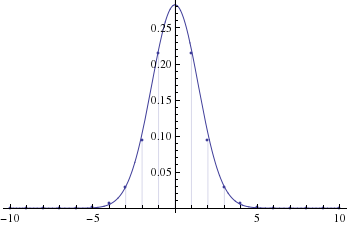
\includegraphics[width=0.3\columnwidth]{diffusion1.png}}
$\lambda t=5${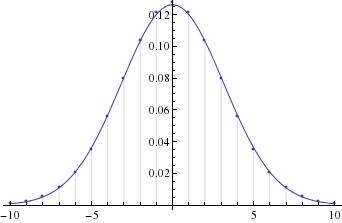
\includegraphics[width=0.3\columnwidth]{diffusion2.png}}
$\lambda t=9${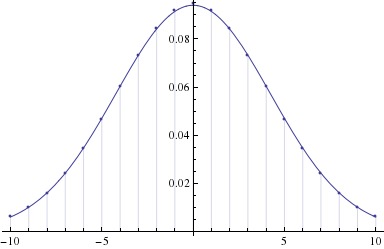
\includegraphics[width=0.3\columnwidth]{diffusion3.png}}
\end{figure}


\noindent
Пользуясь обратным преобразованием Фурье, ответ можно выразить как:
\[
p_{n}(t)=N\int_{-\pi}^{\pi}\frac{dk}{2\pi}\exp(-2\lambda(1-\cos k)t+ikn)
\]


\noindent
Преобразуем интеграл, избавившись от мнимой единицы (вероятность -
величина чисто вещественная). Для этого добавим такой же интеграл
с заменой $k\to-k$ и разделим пополам:
\[
p_{n}(t)=N\int_{-\pi}^{\pi}\frac{dk}{2\pi}\exp(-2\lambda t(1-\cos k))\cos kn
\]


\noindent
Мы получили ответ на вопрос задачи в виде интеграла. Этот интеграл
не берётся в элементарных функциях, однако можно исследовать аналитически
различные асимптотики, используя большое количество методов, изложенных
в этом курсе ранее. Кроме того, его можно исследовать численно (см.
рисунок 1).

\subsection*{Задачи для домашнего решения}

\noindent \textbf{Упражнение 1}

\noindent Вычислите преобразование Фурье следующих функций
\begin{equation}\notag
\frac{\epsilon}{x^{2}+\epsilon^{2}},\quad e^{-|x|/\epsilon},\quad e^{-x^{2}/\epsilon^{2}}.
\end{equation}

\vspace{15pt}
\noindent \textbf{Упражнение 2}

\noindent Пусть $\phi(x)$ - вещественная функция, которая $\rightarrow 0$, при $|x|\rightarrow+\infty$. Докажите следующую формулу:

\begin{equation}\notag
\int_{-\infty}^{+\infty}\phi(x)\left(m^{2}-\frac{d^{2}}{dx^{2}}\right)\phi(x)dx=\int_{-\infty}^{+\infty}\left(m^{2}+k^{2}\right)|\phi(k)|^{2}\frac{dk}{2\pi},
\end{equation}

\noindent где $\phi(k)$ - преобразование Фурье функции $\phi(x)$.

\vspace{15pt}
\noindent \textbf{Упражнение 3}

\noindent Рассмотрите задачу про диффузию на решетке (см. материалы семинара). Приближенно вычислите интеграл, который получился на семинаре для распределения частиц в зависимости от времени

\begin{equation} \notag p_{n}(t)	=N\int_{-\pi}^{\pi}\frac{dk}{2\pi}e^{ikn-2\lambda t(1-\cos k)}
\end{equation}
\noindent в двух предельных случаях: а) $\lambda t\ll 1$, $n$ - фиксированное произвольное число; б) $\lambda t\gg1$.

\vspace{15pt}
\noindent \textbf{Задача 1}

\noindent

\noindent В теории случайных матриц встречаются следующие функции:
\begin{equation}\notag
R_{{\cal U}}(x)	=1-\frac{\sin^{2}x}{x^{2}},\quad R_{{\cal O}}(x)=1-\frac{\sin^{2}x}{x^{2}}+\left[\int_{1}^{+\infty}dz\frac{\sin xz}{z}\right]\cdot\frac{d}{dx}\left(\frac{\sin x}{x}\right).
\end{equation}

\noindent Вычислите их Фурье-преобразования. Результаты изобразите графически.

\vspace{15pt}
\noindent \textbf{Задача 2}

\noindent Функция Бесселя нулевого порядка задается интегралом
\begin{equation}\notag
J_{0}(x)	=\int_{-\pi}^{\pi}\frac{d\phi}{2\pi}\exp\left(ix\sin\phi\right).
\end{equation}

\noindent \textit{Для справки:} при больших значениях аргумента она ведет себя как
\begin{equation}\notag
J_{0}(x	\gg1)=\sqrt{\frac{2}{\pi x}}\cos(x-\pi/4).
\end{equation}

\noindent Вычислите преобразование Фурье функции $J_{0}(x)$ точно. Подумайте, почему особенности в полученном ответе ожидаемы?

\noindent \textbf{Задача 3}

\noindent Рассмотрим самую простую модель твердого тела - цепочку из одинаковых “атомов”, соединенных пружинками.



\noindent Уравнение, которое определяет закон движения атомов в цепочке:
\begin{equation}\notag
m\ddot{u}_{n}	=C(u_{n+1}+u_{n-1}-2u_{n})
\end{equation}
\noindent Здесь $u_{i}$ - смещение атомов от положения равновесия, $m$ - масса одного атома, $C$ - жесткость пружин. Пусть $a$ - расстояние, между атомами в состоянии равновесия. Если подставить в уравнения движения плоскую волну
\begin{equation}\notag
u_{n}	=u_{0}e^{ikan-i\omega t},
\end{equation}
\noindent можно найти закон дисперсии одноатомной цепочки:
\begin{equation}\notag
\omega^{2}(k)	=\frac{4C}{m}\sin^{2}\frac{ka}{2}.
\end{equation}

\noindent Найдите уравнения движения и закон дисперсии “двухатомной” цепочки, т.е. такой же цепочки, как выше, с единственным отличием - массы атомов чередуются как
\begin{equation}\notag
m_{n}	=\begin{cases}
\begin{array}{c}
m\\
M
\end{array} & \begin{array}{c}
n=2l\\
n=2l+1
\end{array}\end{cases}
\end{equation}


\noindent Без ограничений общности считайте, что $M>m$.

\noindent \textit{Подсказка: может быть удобно составить “вектор смещений”}
\begin{equation}\notag
\vec{U}_{l}	=\left(\begin{array}{c}
u_{2l}\\
u_{2l+1}
\end{array}\right).
\end{equation}
\end{document}
